% 例 2：将 BC 沿 v 平移到 B'C'，四边形 BCC'B' 是平行四边形
\documentclass[tikz,border=4pt]{standalone}
\usepackage{ctex}
\usepackage{amsmath}
\usetikzlibrary{calc, arrows.meta, decorations.markings}
\begin{document}
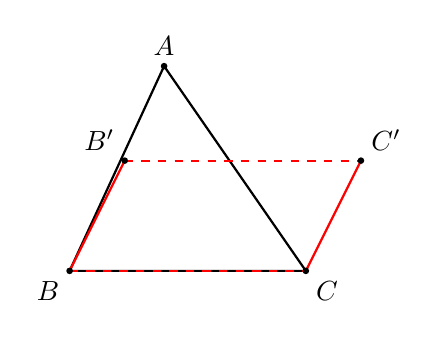
\begin{tikzpicture}[scale=1.0, thick]
  \coordinate (A) at (1.2, 2.6);
  \coordinate (B) at (0, 0);
  \coordinate (C) at (3, 0);
  % 平移向量 v=(0.7, 1.4)
  \coordinate (Bp) at (0.7, 1.4);
  \coordinate (Cp) at (3.7, 1.4);

  \draw (A) -- (B) -- (C) -- cycle;
  \draw[blue, dashed] (Bp) -- (Cp);
  % 平行四边形 BCC'B'
  \draw[red, thick] (B) -- (Bp);
  \draw[red, thick] (C) -- (Cp);
  \draw[red, dashed, thick] (Bp) -- (Cp);
  \draw[red, dashed, thick] (B) -- (C);

  \fill (A) circle (1.2pt); \fill (B) circle (1.2pt); \fill (C) circle (1.2pt);
  \fill (Bp) circle (1.2pt); \fill (Cp) circle (1.2pt);
  \node[above] at (A) {$A$};
  \node[below left] at (B) {$B$};
  \node[below right] at (C) {$C$};
  \node[above left]  at (Bp) {$B'$};
  \node[above right] at (Cp) {$C'$};
\end{tikzpicture}
\end{document}
